\avsnitt{Slutlig design}

En �vergripande modell �ver systemet. L�mpligt format �r ett eller flera klassdiagram, plus eventuella andra modeller som beh�vs f�r att f�rst� hur systemet �r uppbyggt. Diagrammen ska vara l�sbara. Det �r dock fullst�ndigt okej att de �r detaljerade, bara det g�r att zooma in ordentligt p� dem. Ett tips �r att b�rja med ett �versiktligt diagram som inte inneh�ller mer �n paket och klassnamn, och att sedan l�gga till mer detaljerade diagram efter det.

-----------------

Vi valde att dela upp v�rat projekt p� ett s�dant sett att det finns ett separat paket som heter \emph{cards} vilket �r t�nkt som ett allm�nt kortspels-paket med kort, kortlekar, spelare, h�nder osv och sedan ett paket, \emph{texasholdem}, som �r mer specifikt inriktat p� kortspelet Texas Holdem. I det senare ligger ocks� s�dant som mer styr spelregler och spelmekaniken.

Nedan �r ett klassdiagram �ver hela v�rt projekt:\\
\DeclareGraphicsExtensions{.png}
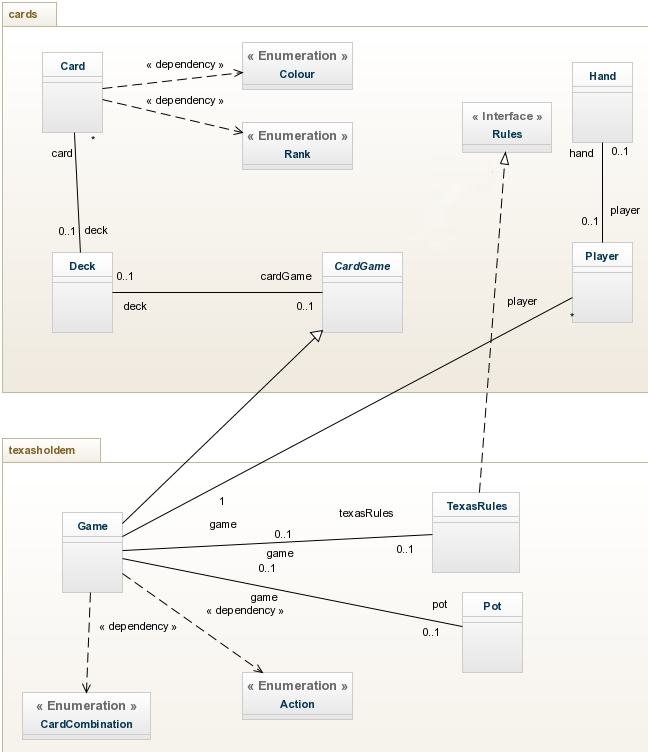
\includegraphics[natwidth=848, natheight=958, scale=0.73, angle=0, trim = 0mm 0mm 42mm 16mm]{bilder/diagram/klassdiagram-2014-10-28}\\
